\section{The Moon-to-Moon Analytical Transfer Method}\label{sec:MMAT}
The MMAT method was created to design tours between the moons of a planet such as Jupiter or
Saturn. However, Canales also demonstrated that it can be similarly applied to interplanetary
transfers by treating the planets as "moons" of the Sun. He provides detailed derivations,
analyses, and examples of the basic MMAT strategy, as well as some extensions relevant to this
investigation\cite{Canales:2021a,Canales:2021b,Canales:2022}. More specifically, the end-to-end
cislunar-Mars transfer methodology presented here employs a distant, two-burn MMAT with a plane
change, bridging the gap between manifolds of Sun-planet CR3BP systems and the true inclinations of
the planetary orbital planes.

\subsection{Methodology}
First, a departure and an arrival CR3BP manifold arc are needed. In this investigation, the
departure CR3BP arc is either a Sun-Earth halo orbit unstable manifold arc or an Earth-Moon orbit
unstable manifold arc propagated within the Sun-Earth dynamics, depending on the transfer category.
Either the departure epoch or the selected manifold arc are varied to determine the departure CR3BP
arc. The arrival CR3BP arc is a Sun-Mars halo orbit stable manifold trajectory. Since an
interplanetary transfer from Earth to Mars is an outward journey, to minimize the $\Delta v$ of the
MMAT solution, the Sun-Mars stable manifold arc with the smallest periapsis (relative to the Sun)
is utilized\cite{Canales:2021b}. For an inward journey, say to Venus, the manifold with the largest
apoapsis is selected, minimizing the Keplerian angular momentum and energy difference between the
departure and arrival CR3BP arcs. The selection process ensures that the departure and arrival
manifold arcs minimize the transfer cost and achieve efficient interplanetary trajectories.

The arcs are propagated under the CR3BP dynamics until they reach a specified distance from their
smaller primary (Earth or Mars), their sphere of influence. Various definitions exist, but for the
MMAT method, the SoI radius is defined as the distance where the ratio of the gravitational
accelerations of the two primaries $d_{SoI}$ is equal to a selected small quantity (see
\cref{eq:patchedSoI})\cite{Canales:2021b}. To ensure that the SoI encompasses most of the Lyapunov
orbit family but also accurately represents when the gravitational effects of that body can be
neglected, the values of $d_{SoI}$ in \cref{tab:SoI} are selected, resulting in their corresponding
radii. Canales provides more details on selecting of appropriate values for
$d_{SoI}$\cite{Canales:2021b}.

\begin{table}[H]
    \centering
    \caption{MMAT sphere of influence radii of relevant CR3BP systems.}
    \begin{tabular}{|c|c|c|}
        \hline
        \textbf{CR3BP System}   &   \boldmath$d_{SoI}$  &   \boldmath$r_{SoI}$  \\  \hline
        Sun-Earth               &   $2.5\times10^{-4}$  &   $0.09877$           \\  \hline
        Sun-Mars                &   $1\times10^{-4}$    &   $0.05375$           \\  \hline
    \end{tabular}
    \label{tab:SoI}
\end{table}

Once the CR3BP manifold arc has reached the edge of the SoI, it is treated as a 2BP trajectory with
the Sun as its focus (refer to the patched 2BP-CR3BP model introduced in \cref{sec:PatchedModels}).
The barycentric rotating frame state that intersects the SoI is transformed to the heliocentric
Ecliptic J2000 frame state applying the procedure outlined in \cref{sec:FrameTransformations}. The
resulting state now defines a Keplerian heliocentric ellipse in the instantaneous plane of motion
of the trajectory at the SoI intersection, the continued path for either the departure or arrival
conic arc. \cref{eq:inclination}-\cref{eq:radialvelocity} are applied to retrieve the equivalent
Keplerian orbital elements. The Keplerian elements fully characterize the heliocentric behavior of
the trajectory, serving as a critical step in connecting the CR3BP manifold dynamics to the
interplanetary transfer framework.

In the distant, two-burn MMAT strategy, for an outward journey, the first maneuver is placed at
the periapsis of the departure conic. Given the true anomaly $\theta=0$ at periapsis,
\cref{eq:eccentricanomaly}-\cref{eq:velocityvector} are applieed to compute the inertial state at
periapsis while \cref{eq:meananomaly} and \cref{eq:Keplersequation} are employed to compute the
time-of-flight along the departure conic:
\begin{equation}
    TOF_{d}=\mathbb{P}_{d}-(t-t_{p}),
    \label{eq:departureTOF}
\end{equation}
where $\mathbb{P}_{d}$ is the period of the departure conic and $(t-t_{p})$ is the time since
periapsis of the SoI state. An inward journey departs from the apoapsis of the departure conic.
The approach aligns the departure conic with the interplanetary bridging trajectory at minimum fuel
cost.

As mentioned previously, a bridge arc is needed to connect the departure and arrival conic arcs,
with a maneuver at both ends. The distant, two-burn MMAT bridge arc for an outward transfer has the
same periapsis radius as the departure conic arc and the same apoapsis as the arrival conic arc
(and vice versa for an inward transfer). The values form a ratio that is utilized to compute the
semimajor axis and eccentricity of the bridge conic:
\begin{equation}
    \mathcal{P}_{b}=\frac{r_{p_{b}}}{r_{a_{b}}}=\frac{1-e_{b}}{1+e_{b}},
    \label{eq:bridgeratio}
\end{equation}
\vspace{1mm}
\begin{equation}
    e_{b}=\frac{1-\mathcal{P}_{b}}{1+\mathcal{P}_{b}},
    \label{eq:bridgeeccentricity}
\end{equation}
\vspace{1mm}
\begin{equation}
    a_{b}=\frac{r_{p_{b}}}{1-e_{b}}.
    \label{eq:bridgesemimajoraxis}
\end{equation}
For an outward journey, the bridge arc lies in the same plane as the departure conic arc, since
Keplerian inclination changes are more efficient the further away they are from the primary,
implying that the remaining three angles of the bridge conic ($i$, $\Omega$, $\omega$) are
identical to those of the departure conic. Since only the semimajor axis and eccentricity change
between the departure and bridge conics, the first maneuver is tangential to the motion at
periapsis, only changing the energy, and is calculated by the difference in the velocity states at
the periapsis. An inward journey combines the inclination change with the first maneuver, so the
bridge conic lies in the same plane as the arrival conic. The following methodology is similar for
the inward case but flipped so that that the constraints are on the intersection between the
departure and bridge conic arcs. The associated equations are also slightly different since the
transfer geometry is flipped. The construction of the bridge arc ensures a smooth and efficient
transition between the departure and arrival conics.

The non-coplanar MMAT methodology revolves around the following analytical constraint derived by
Canales\cite{Canales:2021b}:
\begin{quote}
    As long as the geometrical properties of two conics located in different planes fulfill the
    inequality constraint represented by
    \begin{equation}
        a_{a}(1-e_{a})\leq\frac{a_{b}(1-e_{b}^{2})}{1+e_{b}\cos(\theta_{b_{int}}+n\pi)}\leq a_{a}(1+e_{a}),\text{ being }n=0,1,
        \label{eq:MMAT}
    \end{equation}
    either one of the two conics can be reoriented such that they intersect in space. Consequently,
    the ideal phase of the arrival [planet] at arrival, $\theta_{5_{Mars}}$, for the moon-to-moon
    transfer to occur is obtained considering that the departure epoch, $\theta_{0_{Earth}}$, is
    fixed.
\end{quote}
In the constraint, $\theta_{5_{Mars}}$ and $\theta_{0_{Earth}}$ correspond to $T_{0}$ and $T_{5}$
in \cref{fig:MMAT}. The figure is a schematic of the distant, two-burn MMAT transfer with a plane
change, where the departure and bridge conics are on the same plane but the arrival conic is not.
With the semimajor axes and eccentricities of the bridge and arrival arcs already determined, the
only value still needed for \cref{eq:MMAT} is $\theta_{b_{int}}$, the bridge conic true anomaly at
the intersection location between the bridge and arrival conics ($T_{3}$ in \cref{fig:MMAT}):
\begin{equation}
    \theta_{b_{int}}=u_{b}-\omega_{b},
    \label{eq:bridgeintersect}
\end{equation}
\vspace{1mm}
\begin{equation}
    \sin u_{b}=\frac{\sin(\pi-i_{a})\sin\Delta\Omega}{\sin\psi},
    \label{eq:bridgesinu}
\end{equation}
\vspace{1mm}
\begin{equation}
    \cos u_{b}=\frac{\frac{\sin i_{a}\cos\Delta\Omega}{\cos i_{b}}-\cos\psi\tan i_{b}}{\sin\psi},
    \label{eq:bridgecosu}
\end{equation}
\vspace{1mm}
\begin{equation}
    \cos\psi=\cos i_{a}\cos i_{b}+\sin i_{a}\sin i_{b}\cos\Delta\Omega,
\end{equation}
where $\Delta\Omega=\Omega_{a}-\Omega_{b}$. Note that the value of $n$ that satisfies the
inequality defines the orientation of the bridge conic and is needed later to properly orient the
arrival conic. The center of the inequality in \cref{eq:MMAT} is the intersection distance from the
Sun:
\begin{equation}
    r_{int}=\frac{a_{b}(1-e_{b}^{2})}{1+e_{b}\cos(\theta_{b_{int}}+n\pi)}=\frac{a_{a}(1-e_{a}^{2})}{1+e_{a}\cos(\theta_{a_{int}}+o\pi)}, \text{ being }o=0,1.
    \label{eq:intersect}
\end{equation}
Unfortunately, if the arrival conic arc is not in the same plane as the orbital plane of the
arrival planet, $i_{a}$ and $\Omega_{a}$ cannot be determined prior to the MMAT phasing. As a
result, the arrival phasing needs to be iteratively targeted, making the approach only
semi-analytical. For an initial guess to check the MMAT constraint in \cref{eq:MMAT}, the
inclination and RAAN of the arrival planet orbital plane are selected. The methodology establishes
the foundation for accurately phasing the arrival trajectory in the non-coplanar MMAT framework,
though it requires iterative refinement due to the complexity of aligning orbital planes.

\begin{figure}[H]
    \centering
    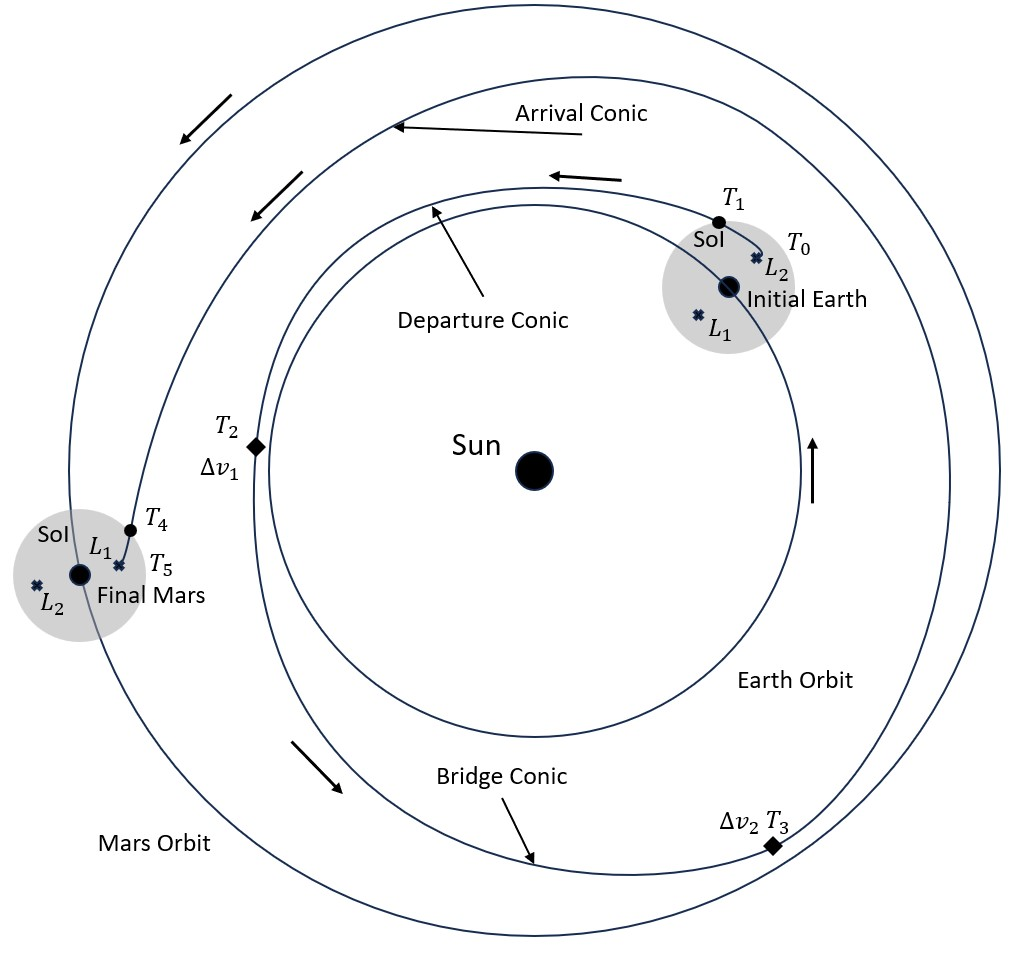
\includegraphics[width=0.75\textwidth]{figures/MMAT.jpg}
    \caption{Representation of the distant, two-burn MMAT with a plane change (adapted from Canales\cite{Canales:2021b}).}
    \label{fig:MMAT}
\end{figure}

The arrival conic true anomaly at the intersection is computed similarly from $r_{int}$, with the
caveat that it is dependent on the arrival phasing and needs to be targeted:
\begin{equation}
    \theta_{a_{int}}=2\pi o+(-1)^{o}\arccos(\frac{\frac{a_{a}(1-e_{a}^{2})}{r_{int}}-1}{e_{a}}),\text{ being }o=0,1.
    \label{eq:arrivalintersect}
\end{equation}
For every feasible $\theta_{b_{int}}$, there are then two possible phasing solutions
($\theta_{a_{int}}$) that correspond to the two arrival ellipse orientations ($\omega_{a}$) that
intersect the bridge ellipse at the line of nodes. A schematic representing the two orientations
appears in \cref{fig:orientation}, where the dashed part of the ellipses are under the $XY$-plane
and the arrows indicate the direction of motion along each ellipse. The angles for the orientation
are calculated similarly to before:
\begin{equation}
    \omega_{a}=u_{a}-(\theta_{a_{int}}+n\pi),
    \label{eq:arrivalperiapse}
\end{equation}
\vspace{1mm}
\begin{equation}
    \sin u_{a}=\frac{\sin i_{b}\sin\Delta\Omega}{\sin\psi},
    \label{eq:arrivalsinu}
\end{equation}
\vspace{1mm}
\begin{equation}
    \cos u_{a}=\cos\Delta\Omega\cos u_{b}+\sin\Delta\Omega\sin u_{b}\cos i_{b}.
    \label{eq:arrivalcosu}
\end{equation}
\cref{eq:arrivalperiapse} is dependent on the orientation of the arrival CR3BP arc, that in turn
depends on a properly phased arrival. Consequently, to solve for the proper phasing and
orientation, an iterative Newton-Raphson differential corrections scheme is applied:
\begin{equation}
    \Xbar=\begin{bmatrix}   \theta_{b_{int}}    &   \theta_{4_{Mars}}   &   \theta_{a_{int}}    \end{bmatrix}^{T},
    \label{eq:MMATfreevar}
\end{equation}
\vspace{1mm}
\begin{equation}
    \Fbar(\Xbar)=\rbar_{a}-\rbar_{b},
    \label{eq:MMATconst}
\end{equation}
where $\theta_{4_{Mars}}$ corresponds to the true anomaly of Mars when the trajectory intersects
the Mars SoI. For an initial guess:
\begin{equation}
    \theta_{4_{Mars}}=\arctan(\cos i_{Mars}\tan\Omega_{Mars})+\omega_{a}+\theta_{a}-(\Omega_{Mars}+\omega_{Mars}+\theta_{Mars_{J2000}})-\arctan(\frac{y_{4}}{|x_{4}|}),
    \label{eq:arrivalepoch}
\end{equation}
where $\theta_{a}$ is the true anomaly of the arrival conic at the SoI intersection,
$\theta_{Mars_{J2000}}$ is the true anomaly of Mars when the Ecliptic J2000 frame is defined, and
$x_{4}$ and $y_{4}$ are the rotating frame coordinates of the trajectory at the SoI intersection.
For the targeting problem, the $DF$ Jacobian matrix is determined with the central difference
method (see \cref{sec:DifferentialCorrections}). Consequently, the iterative process ensures that
the arrival phasing is accurately targeted, enabling a precise transfer solution between the
departure and arrival conics.

\begin{figure}[H]
    \centering
    \includegraphics[width=0.9\textwidth]{figures/orientation.jpg}
    \caption{Representation of the two feasible arrival ellipse orientations. The top images are $XY$-plane views while the bottom are $XZ$-plane views.}
    \label{fig:orientation}
\end{figure}

Once $\Xbar$ has been solved, the true anomaly angles are utilized to compute the Cartesian states
at each location and the times-of-flight of each segment as was done for the departure conic arc.
At the intersection of the bridge and arrival conics, the second maneuver applies an inclination
change on top of the energy change so it is not tangential like the first burn. The $\Delta v$ is
still calculated from the difference in the velocity states at the intersection. The second MMAT
maneuver, incorporating both the energy and inclination changes, completes the transfer.

The transfer solution between the Sun-Earth CR3BP manifold arc and the Sun-Mars CR3BP manifold arc
is now complete. The trajectory is position-continuous throughout, with a maneuver at the beginning
and end of the bridge conic arc to account for the velocity discontinuities. For every feasible
$\theta_{b_{int}}$, there are two corresponding $\theta_{a_{int}}$ that provide transfer solutions.
The two solutions have different maneuver costs and times-of-flight. By continuing in the departure
epoch or the selected manifold arc as discussed, a family of MMAT solutions is obtained and
compared, each offering varying maneuver costs and times-of-flight, that can be further analyzed
based on mission requirements.

\subsection{Example}
What follows is an example MMAT family between a Sun-Earth CR3BP northern halo orbit at a Jacobi
constant of $3.0008189$ and a Sun-Mars CR3BP northern halo orbit at a Jacobi constant of
$3.0001857$. Each transfer in the family starts at a different initial epoch, representing each day
in an Earth year. The initial epochs correspond to $\theta_{0_{Earth}}$ values (that span
0\textdegree-360\textdegree in a year). All of the trajectories utilize the same departure CR3BP
manifold arc, that is the Sun-Earth halo unstable manifold arc with the largest apoapsis,
appearing in \cref{fig:MMATSE}. Similarly, all of the trajectories employ the same Sun-Mars halo
stable manifold arc with the smallest periapsis as the arrival CR3BP arc, appearing in
\cref{fig:MMATSM}. In both figures, the trajectory is propagated to the edge of the sphere of
influence. In between, the departure and arrival conic arcs are determined by the osculating
Keplerian orbital elements when the manifolds reach their respective spheres of influence and the
bridge conic arc joins them as described above, forming a continuous MMAT solution.

In \cref{fig:MMATEvo}(a), the times-of-flight and maneuver magnitudes of the family members appear
with respect to their initial phasing. Note that there are areas of the initial epochs where
transfers could not be computed because the inequality in \cref{eq:MMAT} is not satisfied by those
orientations. Each successful epoch also has two transfer solutions corresponding to the two
arrival phasing solutions described previously. The two groups of transfers in the figure
correspond to the two solutions where $n=0$ or $n=1$ satisfy \cref{eq:MMAT} and are similar due to
the symmetry of the possible bridge conic orientations for an intersection. The full time-of-flight
for the transfers is generally bounded between $3$ and $5.5$ years, while the magnitude of the two
maneuvers combined is between $4$ and $6$ km/s. The analysis highlights the impact of initial
phasing on transfer feasibility and maneuver costs, revealing a range of solutions that satisfy the
MMAT constraints and provide insight into possible interplanetary transfer configurations.

\begin{figure}[H]
    \centering
    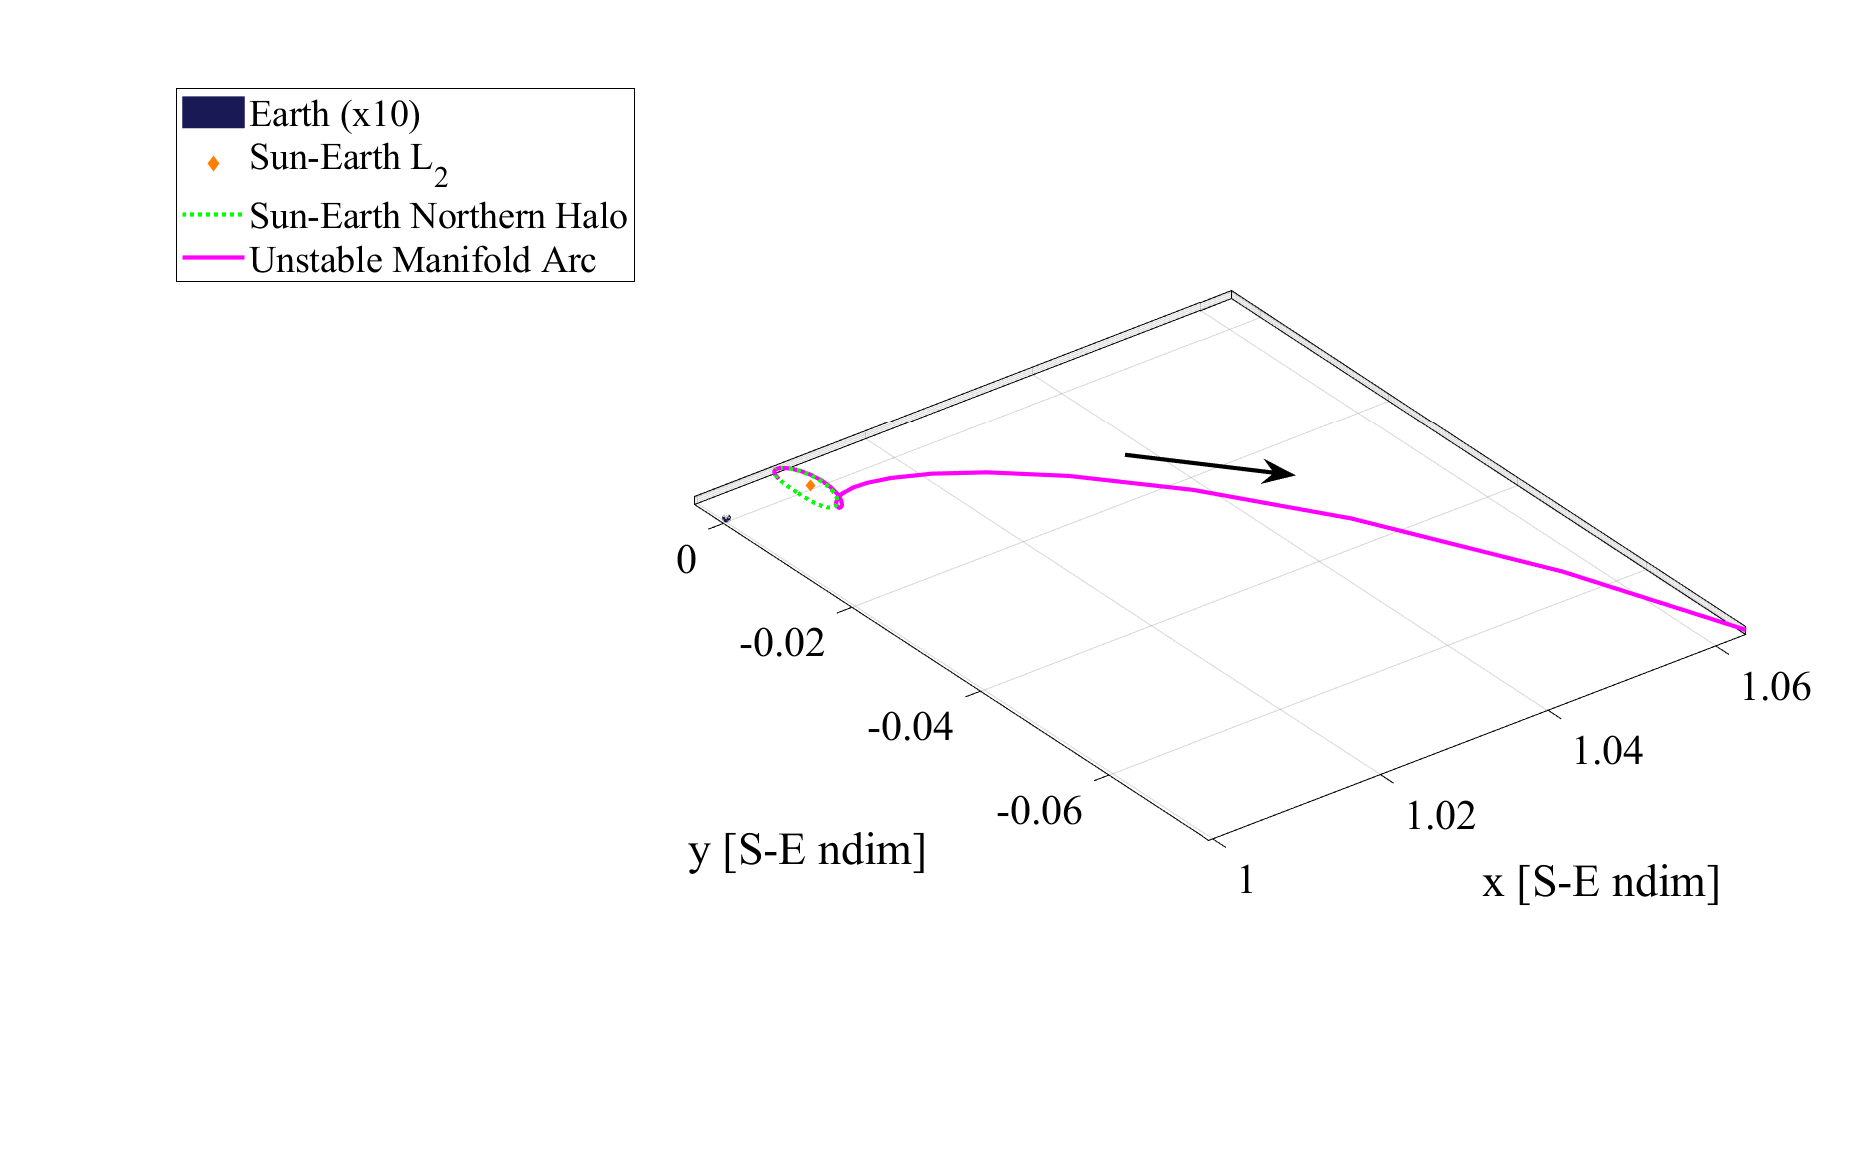
\includegraphics[width=0.9\textwidth]{figures/MinDvSE.pdf}
    \caption{MMAT departure CR3BP arc in the Sun-Earth barycentric rotating frame.}
    \label{fig:MMATSE}
\end{figure}

\begin{figure}[H]
    \centering
    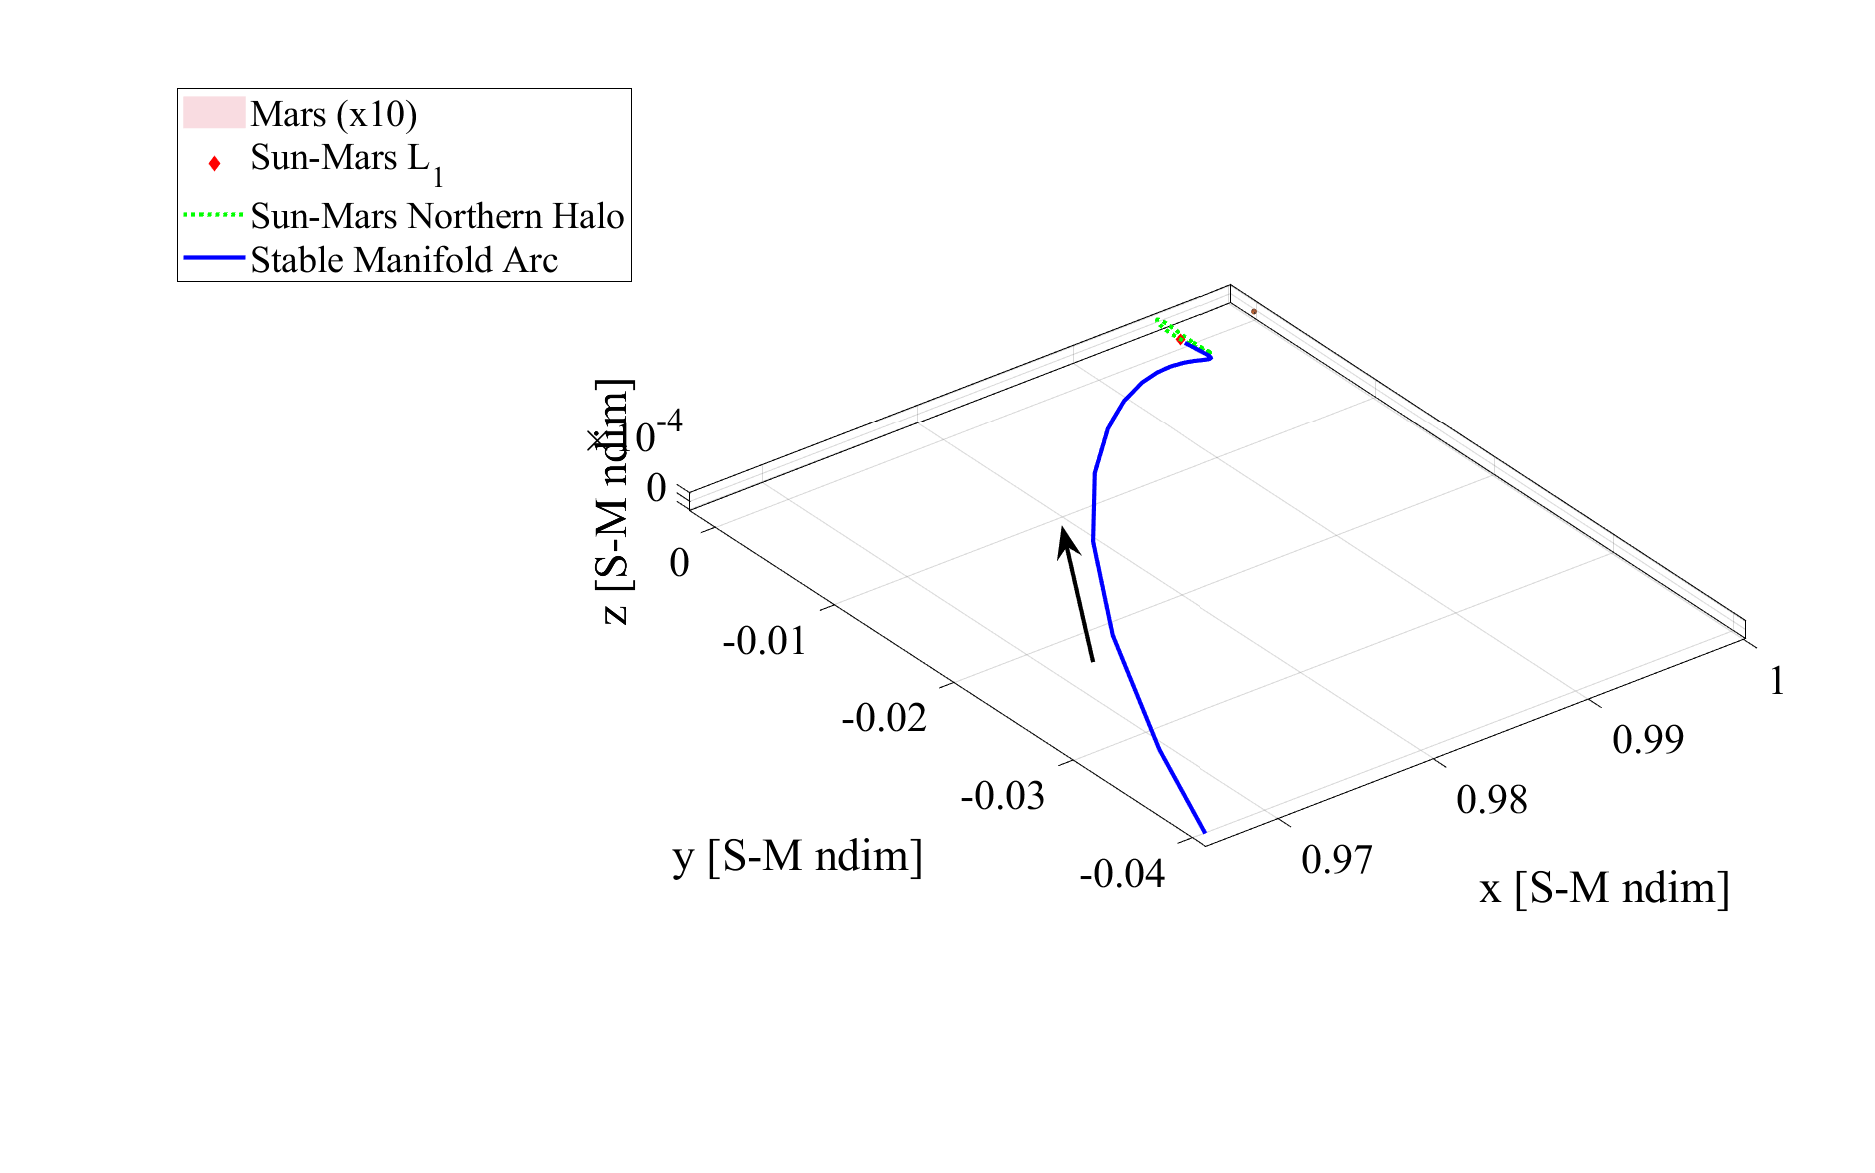
\includegraphics[width=0.9\textwidth]{figures/MinDvSM.pdf}
    \caption{MMAT arrival CR3BP arc in the Sun-Mars barycentric rotating frame.}
    \label{fig:MMATSM}
\end{figure}

\cref{fig:MMATEvo}(b) portrays the same transfers, now with their assosciated initial Mars phasing
$\theta_{0_{Mars}}$. The figure is employed to associate each transfer with an actual launch epoch
where the Earth and Mars are in the specified locations in their respective orbits. Varying the
selected manifold departure arc while keeping the initial epoch fixed creates families that would
appear as vertical lines in \cref{fig:MMATEvo}(b), providing additional launch date flexibility,
potentially at the cost of maneuver $\Delta v$, allowing for a range of transfer solutions, while
emphasizing the trade-off between maneuver cost and timing flexibility.

\begin{figure}[H]
    \begin{subfigure}[h]{0.495\linewidth}
        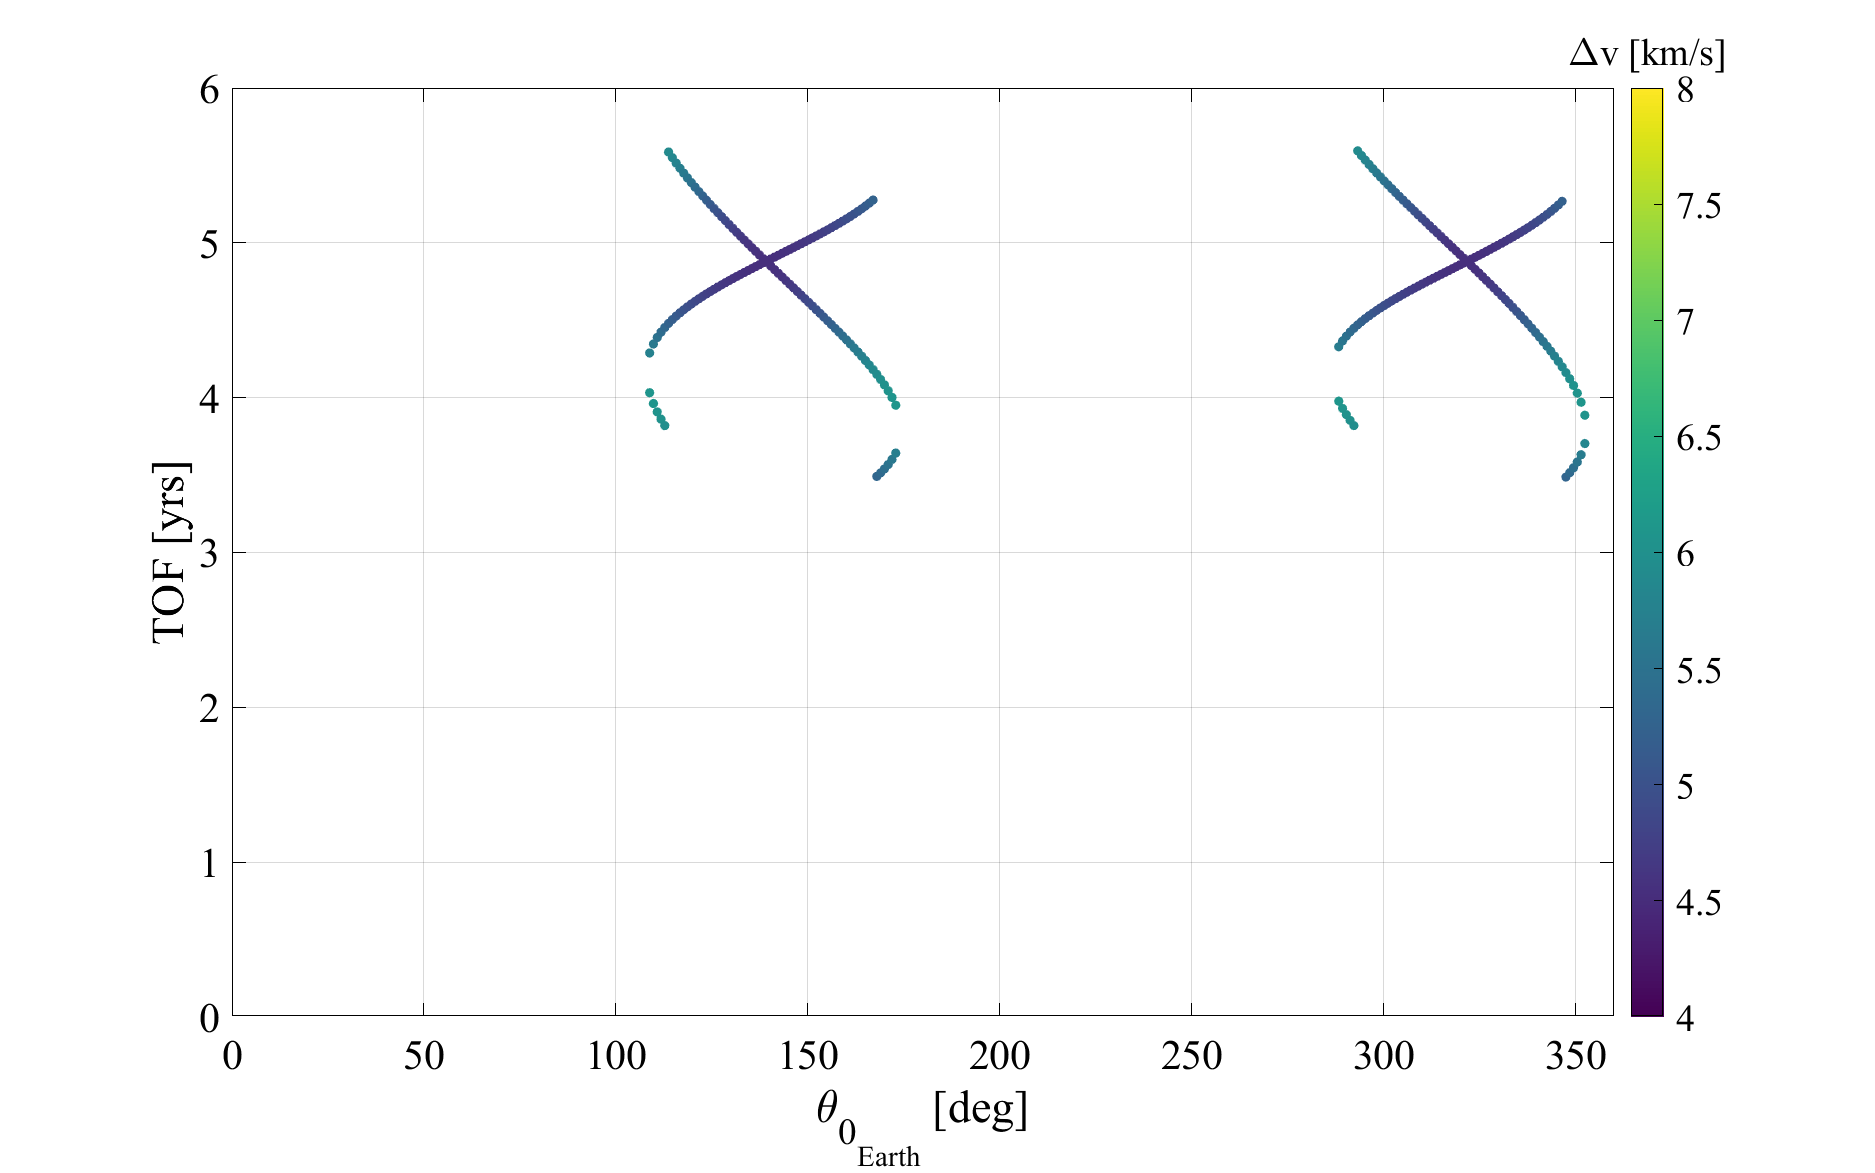
\includegraphics[width=\textwidth]{figures/MMATTOF.pdf}
        \caption{TOF and $\Delta v$}
    \end{subfigure}
    \hfill
    \begin{subfigure}[h]{0.495\linewidth}
        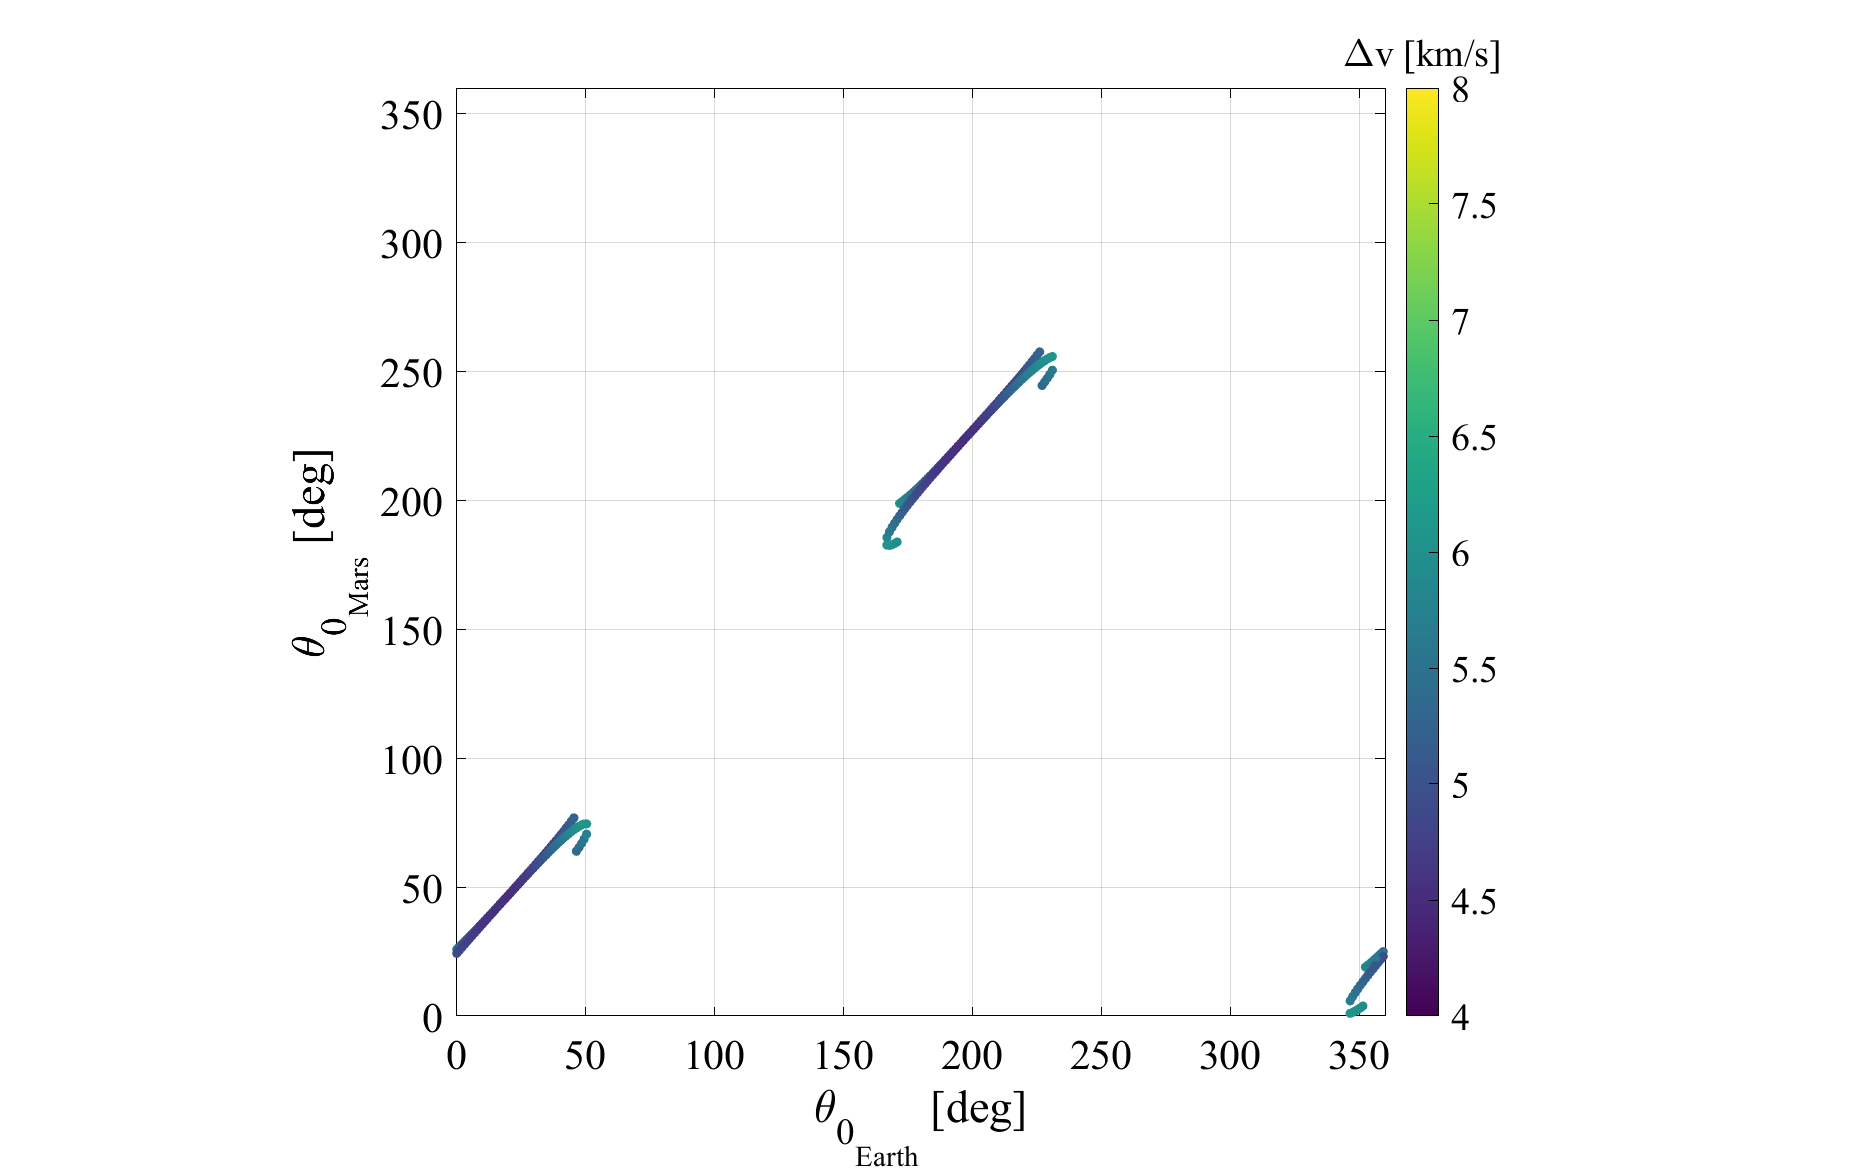
\includegraphics[width=\textwidth]{figures/MMATtheta.pdf}
        \caption{Required planet phasing}
    \end{subfigure}
    \caption{Evolution along the MMAT family continued by the initial epoch.}
    \label{fig:MMATEvo}
\end{figure}

The minimum-$\Delta v$ transfer from the family appears in \cref{fig:MMATDv}. The total TOF of the
transfer is $1670$ days or $4.57$ years, with a total $\Delta v$ of $4.537$ km/s. In the figure,
the various arcs of the MMAT method are color-coded and the maneuvers are marked at the beginning
and end of the bridge conic arc. Note that the magenta departure CR3BP arc and the blue arrival
CR3BP arc are the same trajectories from \cref{fig:MMATSE} and \cref{fig:MMATSM}, respectively,
just portrayed in the Ecliptic J2000 frame. The minimum-$\Delta v$ transfer is compared to the
minimum-TOF transfer in \cref{fig:MMATTOF}. The total TOF has decreased to $1160$ days or
$3.18$ years, but the $\Delta v$ has increased to $5.298$ km/s. Note that the first maneuver has
the same magnitude; the increase comes from the second maneuver where the minimum-TOF burn is less
tangential to the bridge arc than the minimum-$\Delta v$ burn to shorten the arrival conic arc
time-of-flight. All of the other transfers in the MMAT transfer family have similar geometries and
characteristics.

\begin{figure}[H]
    \centering
    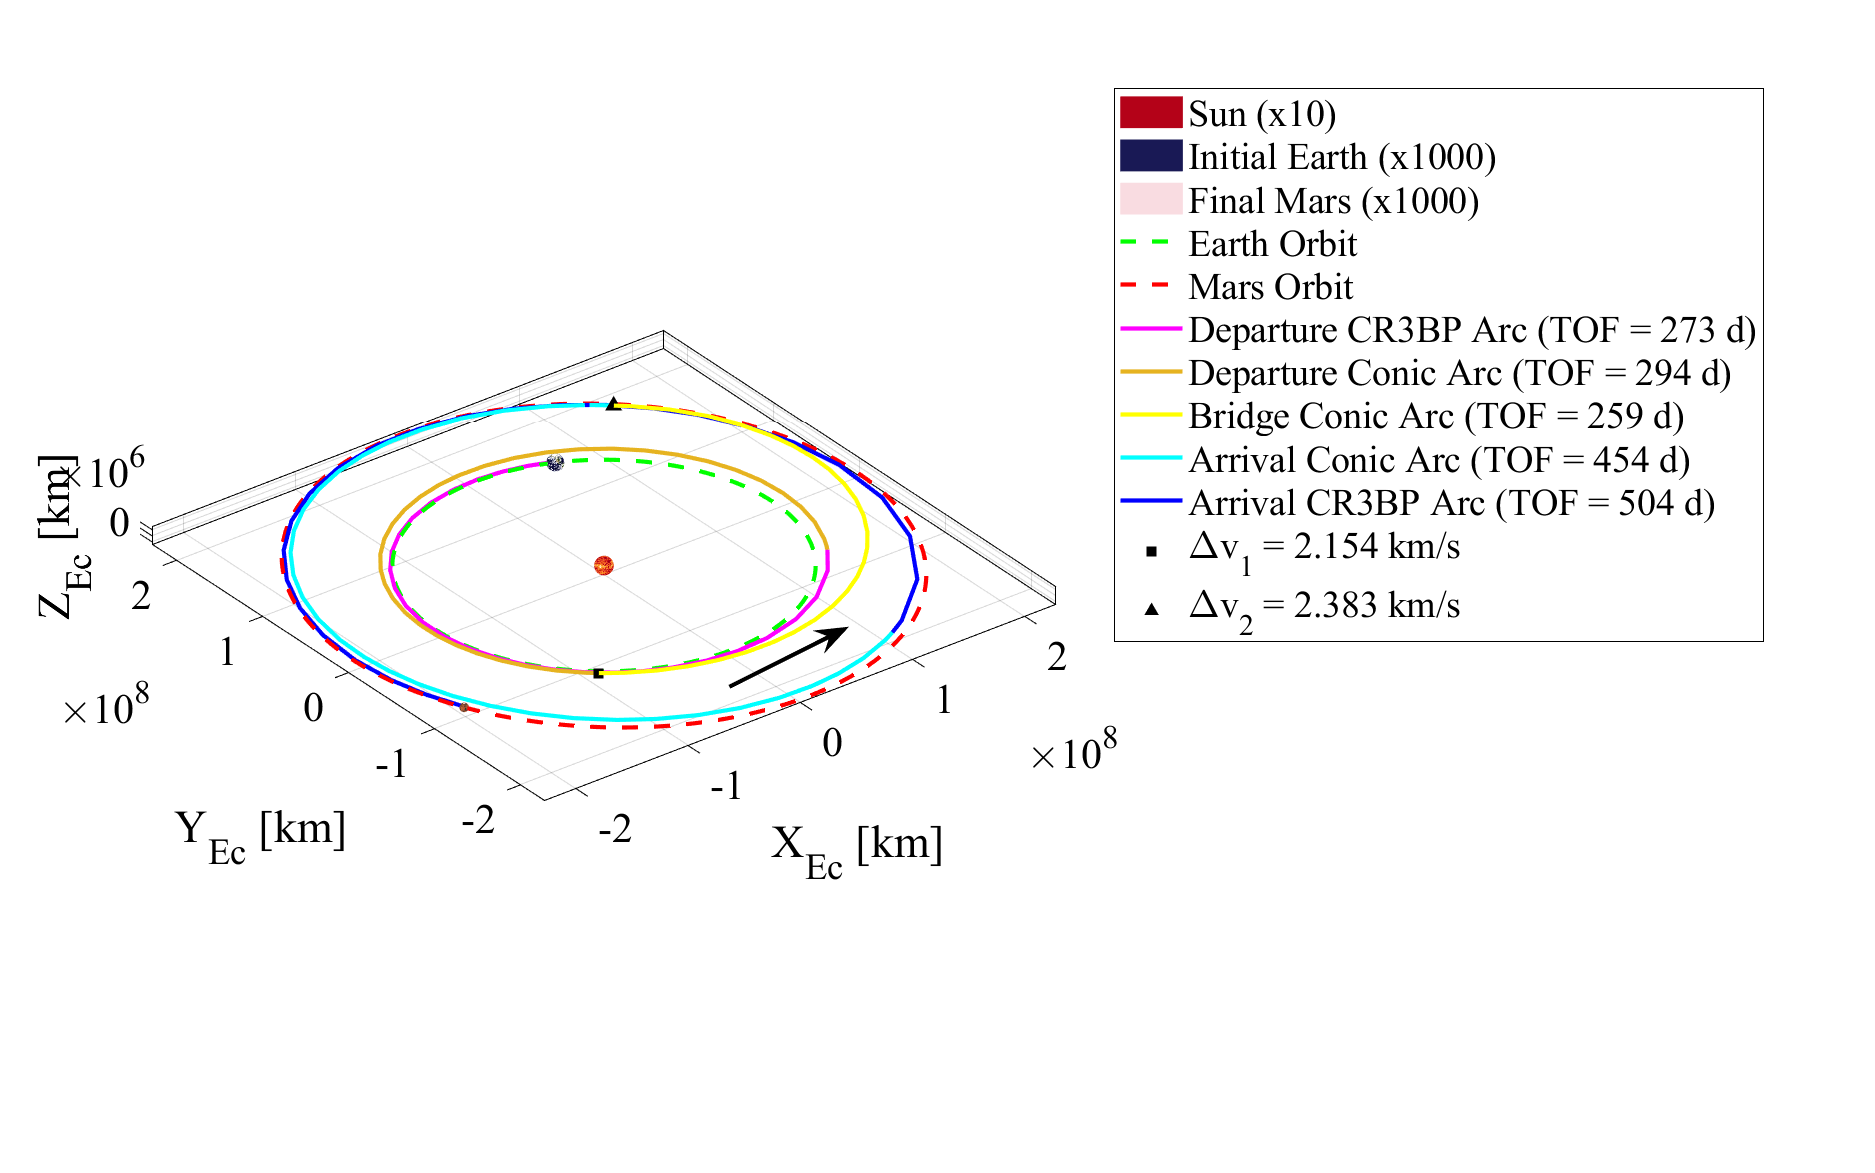
\includegraphics[width=0.9\textwidth]{figures/MinDvMMAT.pdf}
    \caption{Minimum-$\Delta v$ MMAT in the Sun-centered Ecliptic J2000 frame.}
    \label{fig:MMATDv}
\end{figure}

\begin{figure}[H]
    \centering
    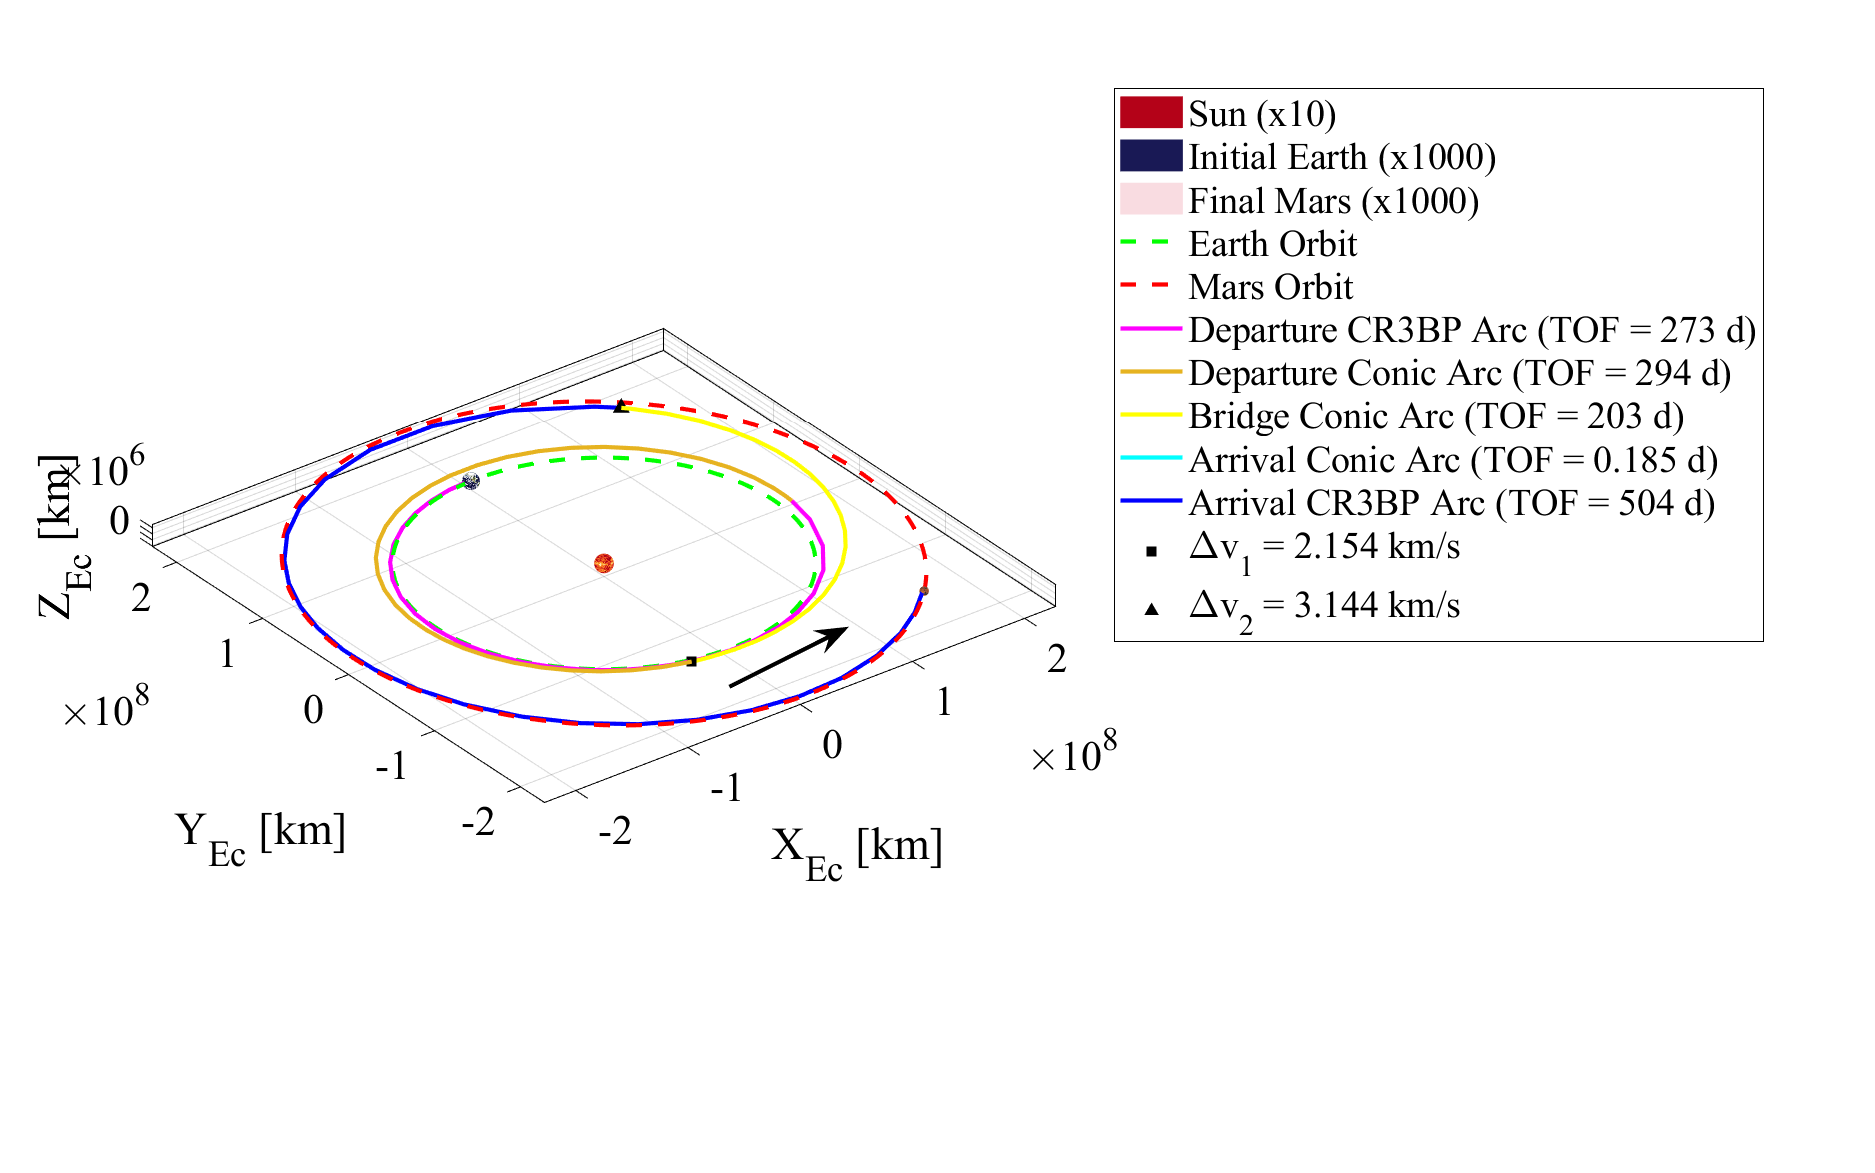
\includegraphics[width=0.9\textwidth]{figures/MinTOFMMAT.pdf}
    \caption{Minimum-TOF MMAT in the Sun-centered Ecliptic J2000 frame.}
    \label{fig:MMATTOF}
\end{figure}
